\chapter{基于主动学习的实体链接语料构建}
本章以无监督学习模型辅助实体链接银标准语料的构建,研究主动学习方法在减少人工标注语料数量上的作用。首先介绍基于图的无监督学习的实体链接方法,包括模型使用的特征以及模型对实体链接任务的处理方法。接着,介绍如何使用主动学习方法选择需要人工辅助标注的样本。最后给出实验结果和实验分析。

\section{基于图的协同推断}
构建语料的常用方法是借助已有模型进行辅助构建,本节将首先给出用于辅助标注实体链接语料的基于图的协同推断方法,这是Han等人\cite{CELWTGBM}提出的一种基于无监督学习的实体链接方法。

在例子“Michael Jordan, the Chicago Bulls retired professional basketball player,  starred in the 1996 feature film Space Jam.”中,已有实体链接方法会通过词袋模型计算指称项“Michael Jordan”和目标实体\textit{Michael Jordan}的相似度,例如实体\textit{Michael Jordan}的维基百科页面摘要中包含“Jordan played 15 seasons in the National Basketball Association (NBA)”,可以看出,由于指称项上下文和实体摘要文本的单词完全不相同,该种方式计算所得的相似度为0。但是“Chicago Bulls”和“NBA”之间却是具有很强的语义关联度的。为了解决这种语义的问题,基于图的协同推断方法借助知识库中的相关信息,建立了实体之间的相关联系,在考虑单个指称项与其对应的候选实体之间的相似度的同时,还考虑了在同一个文档中,不同的指称项之间的候选实体的关联度。

\subsection{实体-实体相似度}\label{section:mm_relation}
同一篇文档中的实体之间一般会有相互关联。在处理实体链接任务时,需要通过定量的方式计算两个实体之间的相似度。张涛等人\cite{张涛2015GraphEL}通过知识库(维基百科)中的链接关系计算实体间的相似度。计算过程中考虑到了其他指称项对应的实体,因而也称为全局相似度。

\begin{figure}[!htb]
	\centering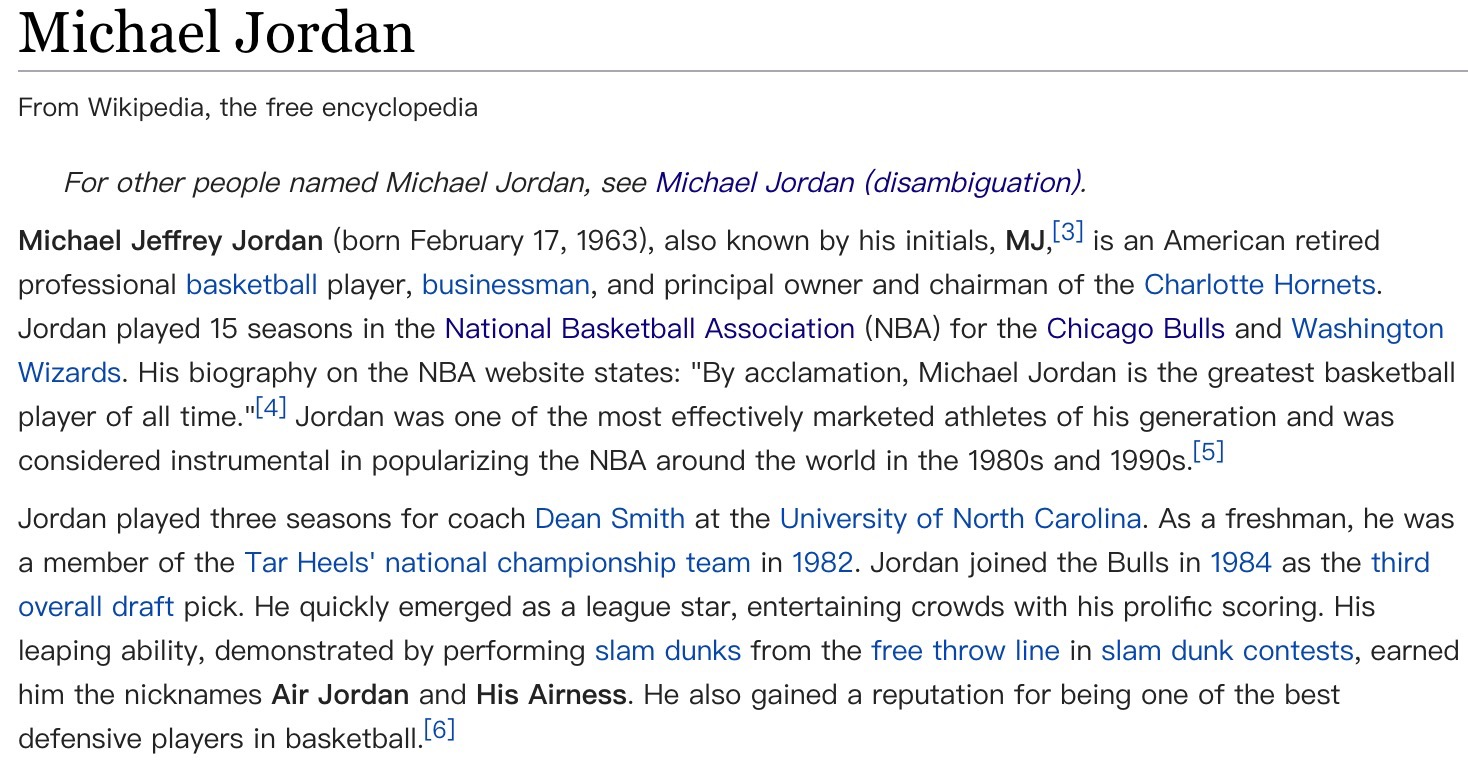
\includegraphics[height=7cm]{resource/jordan_abst}
	\caption{维基百科中\textit{Michael Jordan}的页面}
	\label{fig:jordan_abst}
\end{figure}

图\ref{fig:jordan_abst}是实体\textit{Michael Jordan}在维基百科词条中的部分文本。可以看到,词条文本包含了大量的指向其它实体的链接,例如National Basketball Association、Chicago Bulls、Washington Wizards等。本文通过统计维基百科实体页中的实体链接情况,统计出各个实体在其他实体对应的实体页中被链接的次数,然后计算实体实体之间的相似度,例如,实体$a$和实体$b$之间的相似度可以表示为:

\begin{equation}\label{eq:e_e_relation}
SR(a,b)=1-\frac{\log (\max(|A|,|B|))-\log(|A\cap B|)}{\log(|W|)-\log(\min(|A|,|B|))}
\end{equation}

公式\ref{eq:e_e_relation}中,$A$和$B$分别表示维基百科中对应实体页中包含链接到实体$a$和实体$b$的实体集合。$W$表示维基百科中所有实体的集合。在示例文本中,包含“Michael Jordan”、“Chicago Bulls”、“Space Jam”这三个指称项,其中“Michael Jordan”指向的实体可能是\textit{Michael Jordan},也可能是\textit{Michael B. Jordan}。计算这两个实体和其它两个指称项对应的实体之间的相似度,结果如表\ref{tab:ee_relation_example}所示。

\begin{table}[!htb]
	\caption{实体间相似度例子\label{tab:ee_relation_example}}
	\centering
	\begin{tabular}{|c|c|c|}
		\hline
		 & Space Jam & Chicago\\
		\hline
		Michael Jordan & 0.66 & 0.82\\
		\hline
		Michael B. Jordan & 0.00 & 0.00\\
		\hline
	\end{tabular}
\end{table}

观察该表可以发现,当确定文本中指称项“Chicago Bulls”和“Space Jam”所指向的实体分别是\textit{Chicago Bulls}和\textit{Space Jam}之后,计算\textit{Michael Jordan}与\textit{Chicago Bulls}、\textit{Space Jam}的实体相似度分别是$0.66$和$0.82$,\textit{Michael B. Jordan}与\textit{Chicago Bulls}、\textit{Space Jam}的实体相似度都是$0.00$。由此可以推断,\textit{Michael Jordan}与上下文环境的实体相似度更大,更有可能是指称项“Michael Jordan”对应的目标实体。

\subsection{指称项-实体相似度}\label{section:me_relation}
指称项-实体相似度是指在给定指称项$m$和候选实体$e$后,根据指称项$m$上下文等特征计算得到的和候选实体$e$之间的相似度。计算相似度时,因为只考虑单个指称项,因而也称为局部相似度。

计算指称项-实体相似度需要为指称项的上下文定义一个窗口大小,通过计算该窗口文本和候选实体词条摘要文本的相似度得到指称项-实体相似度。本文参考Pedersen等人\cite{pedersen2005name}的相关研究,将上下文的窗口大小定义为50。

本文采用词袋模型计算指称项-实体相似度,给定指称项$m$和候选实体$e$,指称项-实体相似度如公式\ref{eq:m_m_relation}所示:

\begin{equation}\label{eq:m_m_relation}
CP(m,e)=\frac{m\cdot e}{|m||e|}\\
\end{equation}

其中,$m$和$e$分别是指称项窗口文本和候选实体知识库摘要文本的词向量表示,向量中的每个维度分别是对应单词的TFIDF表示。

\subsection{构建协同推断图}\label{section:ref_graph}
协同推断图的每个节点可以是指称项,也可以是指称项对应的候选实体。图中的边分为两种类型,第一类是指称项节点和候选实体节点之间的边,这类边的权值用指称项-实体相似度表示。第二类是候选实体节点和其它候选实体节点之间的边,这类边的权值用实体-实体相似度表示。由于一个指称项对应的候选实体集包含的候选实体数量可能非常大,那么协同推断图的节点和边的数量可能也会非常大。图的复杂度太高会直接影响后续在图上相关计算的效率,为了解决这个问题,本文对连接边权值较小的候选实体节点和边做了删除处理。

\begin{figure}[!htb]
	\centering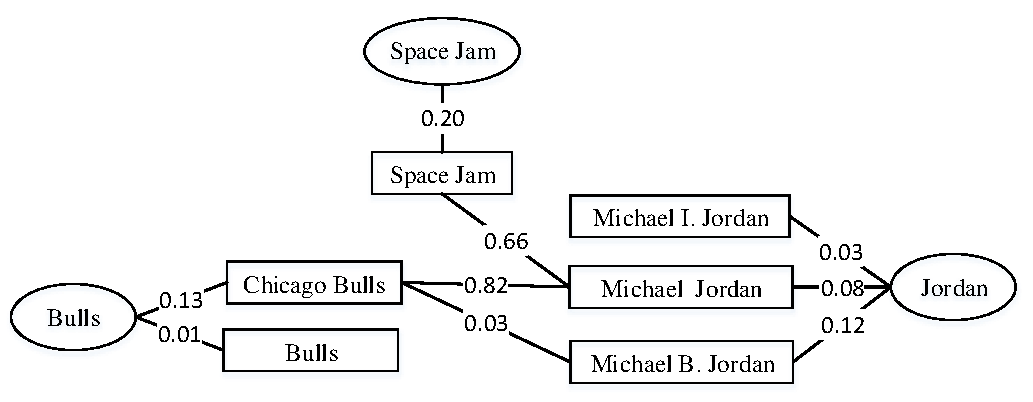
\includegraphics[height=5cm]{resource/EL_Graph}
	\caption{协同推断图示例图}
	\label{fig:el_graph}
\end{figure}

图\ref{fig:el_graph}是实体链接任务中协同推断图的一个例子。图中椭圆边框的节点表示指称项,矩形边框的节点表示指称项对应的候选实体。例如指称项“Jordan”的候选实体包含\textit{Michael I. Jordan}、\textit{Michael Jordan}、\textit{Michael B. Jordan}。指称项“Jordan”与其对应的候选实体之间的边的权值是指称项和实体之间的局部相似度。不同指称项对应的候选实体之间的边为全局相似度,例如指称项“Jordan”对应的候选实体\textit{Michael Jordan}和指称项“Bulls”的候选实体\textit{Chicago Bulls}的实体相似度为0.82。图中并非所有节点都有连接边,这是因为一些边的权值很小,为提高后续计算效率而被删除。

\subsection{协同推断方法}\label{section:collective_infer_method}
构建好协同推断图以后,通过随机行走(Random Walk, RW)算法\cite{tong2006fast}对候选实体的置信度进行推断,选择置信度最高的候选实体作为预测目标实体。

协同推断图中包含$n$个节点($k$个指称项节点和$l$个候选实体节点)。首先需要计算文本中所有指称项在上下文中的重要程度,如公式\ref{eq:m_importance}所示。

\begin{equation}\label{eq:m_importance}
Importance(m)=\frac{tfidf(m)}{\sum_{m\in D} tfidf(m)}\\
\end{equation}

初始证据向量$s$的维度为$k+l$,对$s$的初始化方法如公式\ref{eq:init_evidence}所示。

\begin{equation}\label{eq:init_evidence}
s_i=\left\{
\begin{array}{rcl}
Importance(m)       &      & {\text{节点}i\text{对应指称项}m}\\
0    &      & {\text{节点}i\text{对应候选实体}}
\end{array} \right.
\end{equation}

证据传递矩阵$T$是一个大小为$(k+l)\times (k+l)$的矩阵。该矩阵是一个稀疏矩阵,定义如公式\ref{eq:prob_trans_maze}所示。公式中$E_m$表示指称项$m$对应的候选实体集,$N_e$表示推断图中与实体$e$有边相连的实体集合。

\begin{equation}\label{eq:prob_trans_maze}
T_{ij}=\left\{
\begin{array}{rcl}
\frac{CP(m,e)}{\sum_{e\in E_m} CP(m,e)}       &      & {\text{节点}j\text{对应指称项}m\text{,节点}i\text{对应候选实体}e}\\
\frac{SR(e_i,e_j)}{\sum_{e\in N_{e_j} SR(e_i,e)}}    &      &{\text{节点}j\text{对应候选实体}e_j\text{,节点}i\text{对应候选实体}e_i}\\
0    &      &{\text{其它}}\\
\end{array} \right.
\end{equation}

在实体链接任务中,随机行走算法如算法\ref{algorithm_random_walk}所示。

\floatname{algorithm}{算法}
\renewcommand{\algorithmicrequire}{\textbf{输入:}} % Use Input in the format of Algorithm
\renewcommand{\algorithmicensure}{\textbf{输出:}} % Use Output in the format of Algorithm
\begin{algorithm}[!htb]
	\caption{基于图的协同推断中的随机行走算法}
	\label{algorithm_random_walk}
	\begin{algorithmic}[1] %这个1 表示每一行都显示数字
		\REQUIRE ~ %算法的输入参数:Input
		初始证据向量$s$,证据传递矩阵$T$
		\ENSURE ~ %算法的输出:Output
		图的稳定状态证据向量$r^*$
		\STATE 初始化$r^0=s$
		\REPEAT
		\STATE $r^{t+1}=(1-\lambda)\times T\times r^t + \lambda \times s$\label{random_walk_iter}
		\UNTIL {$r$得到稳定状态或者迭代次数达到上限}\label{random_walk_stop_condition}
		\RETURN $r^*$
	\end{algorithmic}
\end{algorithm}

由于$T$是一个稀疏矩阵,协同推断图中存在一些候选实体节点没有出边,因此算法\ref{algorithm_random_walk}的第\ref{random_walk_iter}行,在随机行走的迭代过程中,加入了证据重分配率参数$\lambda$\footnote{本文通过实验,取$\lambda=0.5$,效果最佳。},这是为了在随机行走过程中以一定概率从起始点重新进行随机行走,解决某些节点无法进行证据传播的问题。参考Hu等人\cite{hu2009understanding}的相关研究,算法第\ref{random_walk_stop_condition}行的迭代次数上限,本文选取的值为100。

以图\ref{fig:el_graph}为例,初始证据向量$s=\left( 0.41,0.33,0.26,0,0,0,0,0,0\right)^T $,$r^0=s$。随机行走过程第1次迭代如公式\ref{eq:random_walk_iter1}所示。

\begin{equation}\label{eq:random_walk_iter1}
\left(
\begin{matrix}
0.21\\
0.17\\
0.13\\
0.03\\
0.07\\
0.11\\
0.15\\
0.01\\
0.13\\
\end{matrix}
\right)
=.5\times
\left(
\begin{matrix}
0 & 0 & 0 & 0 & 0 & 0 & 0 & 0 & 0\\
0 & 0 & 0 & 0 & 0 & 0 & 0 & 0 & 0\\
0 & 0 & 0 & 0 & 0 & 0 & 0 & 0 & 0\\
0.13 & 0 & 0 & 0 & 0 & 0 & 0 & 0 & 0\\
0.35 & 0 & 0 & 0 & 0 & 0 & 0.96 & 0 & 0\\
0.52 & 0 & 0 & 0 & 0 & 0 & 0.04 & 0 & 0\\
0 & 0.92 & 0 & 0 & 0.55 & 1 & 0 & 0 & 0\\
0 & 0.08 & 0 & 0 & 0 & 0 & 0 & 0 & 0\\
0 & 0 & 1 & 0 & 0.45 & 0 & 0 & 0 & 0\\
\end{matrix}
\right)\times
\left(
\begin{matrix}
0.41\\
0.33\\
0.26\\
0\\
0\\
0\\
0\\
0\\
0\\
\end{matrix}
\right)+
.5\times
\left(
\begin{matrix}
0.41\\
0.33\\
0.26\\
0\\
0\\
0\\
0\\
0\\
0\\
\end{matrix}
\right)
\end{equation}

在完成第100轮随机行走迭代过程后,达到了稳定状态下,最后一轮迭代如公式\ref{eq:random_walk_iter100}所示。

\begin{equation}\label{eq:random_walk_iter100}
\left(
\begin{matrix}
0.21\\
0.17\\
0.13\\
0.01\\
0.10\\
0.06\\
0.13\\
0.01\\
0.09\\
\end{matrix}
\right)
=.5\times
\left(
\begin{matrix}
0 & 0 & 0 & 0 & 0 & 0 & 0 & 0 & 0\\
0 & 0 & 0 & 0 & 0 & 0 & 0 & 0 & 0\\
0 & 0 & 0 & 0 & 0 & 0 & 0 & 0 & 0\\
0.13 & 0 & 0 & 0 & 0 & 0 & 0 & 0 & 0\\
0.35 & 0 & 0 & 0 & 0 & 0 & 0.96 & 0 & 0\\
0.52 & 0 & 0 & 0 & 0 & 0 & 0.04 & 0 & 0\\
0 & 0.92 & 0 & 0 & 0.55 & 1 & 0 & 0 & 0\\
0 & 0.08 & 0 & 0 & 0 & 0 & 0 & 0 & 0\\
0 & 0 & 1 & 0 & 0.45 & 0 & 0 & 0 & 0\\
\end{matrix}
\right)\times
\left(
\begin{matrix}
0.21\\
0.17\\
0.13\\
0.01\\
0.10\\
0.06\\
0.13\\
0.01\\
0.09\\
\end{matrix}
\right)+
.5\times
\left(
\begin{matrix}
0.41\\
0.33\\
0.26\\
0\\
0\\
0\\
0\\
0\\
0\\
\end{matrix}
\right)
\end{equation}

对于给定的指称项$m$,基于图的协同推断方法用公式\ref{eq:collective_inference}计算$m$对应的预测目标实体。其中$r(e)$是随机行走达到稳定状态后,候选实体$e$通过图推断后得到的评分,与局部相似度$CP(m,e)$相乘后得到综合评分,并取指称项$m$对应的候选实体集中,综合评分最高的候选实体作为$m$的预测目标实体。

\begin{equation}\label{eq:collective_inference}
m.e^*=\argmax_e CP(m,e)\times r(e)
\end{equation}

\begin{table}[!htb]
	\caption{主动学习策略结果评价\label{tab:el_graph_score}}
	\centering
	\begin{tabular}{|c|c|c|c|}
		\hline
		\textbf{候选实体} & \textbf{Michael I. Jordan} & \textbf{Michael Jordan} & \textbf{Michael B. Jordan}\\
		\hline
		$r(e)$ & 0.01 & 0.10 & 0.06\\
		\hline
		\textbf{候选实体} & \textbf{Chicago Bulls} & \textbf{Bulls} & \textbf{Space Jam}\\
		\hline
		$r(e)$ & 0.13 & 0.01 & 0.09\\
		\hline
	\end{tabular}
\end{table}

表\ref{tab:el_graph_score}给出了本节的例子中,各个候选实体在随机行走达到稳定状态后的推断评分。通过观察可以发现,经过协同推断进程后,候选实体\textit{Michael Jordan}、\textit{Chicago Bulls}、\textit{Space Jam}是在其对应的指称项的候选实体集里面推断评分最高的,通过公式\ref{eq:collective_inference}计算得到的综合评分也是最高的,验证了基于图的协同推断方法的有效性。

\section{银标准语料构建方法}
银标准语料即存在错误标注,但不会对模型训练产生很大影响的语料。在成本有限的情况下,提高银标准语料质量对模型训练有重要意义。虽然Han等人\cite{CELWTGBM}通过实验证明了基于图的协同推断方法是目前性能较好的实体链接方法,但是该方法在本文所使用的数据集上仅能达到73.3\%的正确率。其在正确率上距离高质量银标准语料还有一定差距。常用的方法是人工对部分未标注样本进行标注,然后通过已标注样本对未标注样本进行证据传播,从而提高其它未标注样本的预测精度。

在人工标注并证据传播的过程中,有以下两个关键问题:

(1)如何从未标注指称项样本中选择需要交由人工标注的待标注样本。

(2)对指称项对应的目标实体进行标注以后,如何影响其它未标注样本的目标实体预测。

本文将在以下两节分别介绍待标注指称项的选择方法和已标注指称项的证据传播方法。

\subsection{待标注指称项选择方法}\label{section:anno_select}
以下是四种待标注指称项选择方法,其中第一种采用顺序选择方法,后三种都是基于主动学习的选择方法。

\subsubsection{顺序指称项选择法}
该方法是一种基线方法。对一篇文档$D$中的所有指称项$M=\{m_1,m_2,...,m_n\}$,按照指称项出现的先后顺序对指称项进行标注。

该方法的优点在于实现简单,并且顺序标注符合人的标注习惯。该方法的缺点是,当实体链接模型性能较高的时候,提交人工标注的指称项有很大概率已经被正确预测,增加人工标注的工作量,标注效率较低。

\subsubsection{最大不确定度的指称项选择法}\label{section:margin_select}
该方法利用基于间隔的主动学习方法对待标注指称项进行了选择。对于给定指称项$m$及其候选实体集合$E_m$,对$E_m$中的每个候选实体$e$的综合评分做归一化处理,得到候选实体$e$是目标实体的置信度,如公式\ref{eq:el_graph_prob}所示。

\begin{equation}\label{eq:el_graph_prob}
P(e|m)=\frac{CP(m,e)\times r(e)}{\sum_{e\in E_m}CP(m,e)\times r(e)}
\end{equation}

通过公式\ref{eq:el_graph_confidence}计算指称项$m$的候选实体中综合评分最高的两个候选实体的置信度的差的绝对值,以此作为指称项$m$被正确链接的置信度。
\begin{align}\label{eq:el_graph_confidence}
\begin{aligned}
	Confidence(m)&=P(e^{*1}|m)-P(e^{*2}|m)\\
	\text{其中,\quad\quad\quad\quad\quad\quad\quad\quad\quad\quad\quad}&\text{\quad\quad\quad\quad\quad\quad\quad\quad\quad\quad\quad\quad\quad\quad\quad\quad\quad}\\
	e^{*1}&=\argmax_{e_i\in E_m}P(e_i|m)\\
	e^{*2}&=\argmax_{e_i\in E_m \setminus e^{*1}}P(e_i|m)
\end{aligned}
\end{align}

得到指称项$m$被正确链接的置信度以后,通过公式\ref{eq:el_graph_uncertainty}计算指称项$m$链接的不确定度。
\begin{equation}\label{eq:el_graph_uncertainty}
Uncertainty(m)=1-Confidence(m)
\end{equation}

链接不确定度越大的指称项,预测标注错误的可能性越大。因此,在每一轮待标注样本选择过程中,需要选择链接不确定度最大的指称项交由人工标注,通过这种方式尽可能找出错误预测的指称项,从而提高人工标注的效率。

\subsubsection{基于同名指称项的最大标注回报选择法}
该方法在利用主动学习方法选择待标注样本的过程中,不仅考虑到了样本的不确定度,同时也考虑到了样本的代表性。在同一篇文档中,相同的指称项可能出现多次,这些指称项很可能指向同一个实体。对这些指称项中的某一个指称项做人工标注,可以提高其它指称项预测的正确率。这里,对指称项$m$进行标注的回报率进行评估时,评估结果由与$m$同名的指称项集合$M_m=\{m^{'}|Name_m=Name_{m^{'}}\}$中的所有指称项共同确定,如公式\ref{eq:dupName_uncartainty}所示。

\begin{equation}\label{eq:dupName_uncartainty}
Reward(M_m)=\sum_{m^{'}\in M_m} {Uncertainty(m^{'})}
\end{equation}

从公式中可以直观地看出,同一文档中,同名指称项出现的次数越多,各个指称项链接的不确定度越大,则对指称项进行人工标注的回报率越大。对$Reward(M_m)$值最大的指称项集合$M_m$中的某个指称项进行人工标注,理论上对语料库实体链接预测正确率的提升效果最大。

\subsubsection{基于相似指称项的最大标注回报选择法}
存在一些指称项集合,它们存在共指关系,但是它们名字的字符串并不是严格相等的,可能是缩写、别名等其它形式。例如在同一篇文档中,指称项“Microsoft”和指称项“MS”可能就是全名和缩写的关系,它们所指向的实体是相同的。基于字符串完全匹配的方法的缺点是无法利用这类指称项之间的共指关系。

为了克服上述缺点,本文提出了基于相似指称项的最大标注回报选择方法。本文通过知识库相关信息抽取得到候选实体词典,然后借助候选实体词典,根据指称项对应的候选实体集计算不同指称项之间的语义相似度。

\begin{equation}\label{eq:mention_semi}
MS(m_1,m_2)=\frac{|E_{m_1}\cap E_{m_2}|}{\min(|E_{m_1}|,|E_{m_2}|)+0.1}
\end{equation}

公式\ref{eq:mention_semi}是指称项$m_1$和指称项$m_2$之间语义相似度的计算方法。该公式的假设是,相同或相似的指称项,对应的候选实体集相似度也应该会更高。在极端情况下,两个相同的指称项,候选实体集完全相同,指称项之间的语义相似度为1。相反,完全不相关的指称项,对应的候选实体集交集为空,则指称项之间的语义相似度为0。

因此,在评估指称项$m$的标注回报率时,评估结果由与$m$相似的指称项集合$M_m=\{m^{'}|MS(m,m^{'})>=\alpha\}$(公式中的$\alpha$通过实验获得,本文取值为0.8)中的所有指称项共同确定,计算方式与公式\ref{eq:dupName_uncartainty}相同,也是由指称项集合$M_m$中的所有指称项链接不确定度的和得到。

同样地,选择需要人工标注的指称项时,也是需要从$Reward(M_m)$最大的指称项集合中取出一个指称项进行标注,这里从集合中选取的原则是选择不确定度最大的指称项。

\subsection{已标注指称项证据传播方法}\label{section:anno_propagate}
同一篇文档会包含多个指称项,一方面,这些指称项通常会有相互关联的关系,例如同一篇文档中既包含“Jordan”这个指称项,又包含“Bulls”这个指称项。如果人工标注“Jordan”指向\textit{Michael Jordan}这个实体,那么“Bulls”则很可能指向\textit{Chicago Bulls}这个实体。另一方面,采用基于同名指称项的最大标注回报选择法和基于相似指称项的最大标注回报选择法时,经过人工标注的指称项会对文档中的其它未标注指称项的目标实体预测产生一定的影响。

在同一篇文档中,相同或者相似的指称项可能会出现多次,例如出现多个“Jordan”指称项,当人工标注其中一个“Jordan”指向\textit{Michael Jordan}这个实体,那么其它“Jordan”指称项很可能也指向\textit{Michael Jordan}这个实体。另外还需要考虑到不同字符串表示的指称项可能存在共指关系,即它们可能指向同一个实体,例如指称项“Jordan”和指称项“Michael Jordan”如果出现在同一篇文档中,则它们也很可能指向同一个实体\textit{Michael Jordan}。

\subsubsection {图的迭代推断}
当标注者标注指称项$m$指向实体$e$以后,需要对协同推断图做以下处理。首先,需要删除指称项$m$对应的候选实体集$E_m$中除目标实体$e$以外的其他候选实体节点。然后删除与被移除节点相连的边。

\begin{figure}[!htb]
	\centering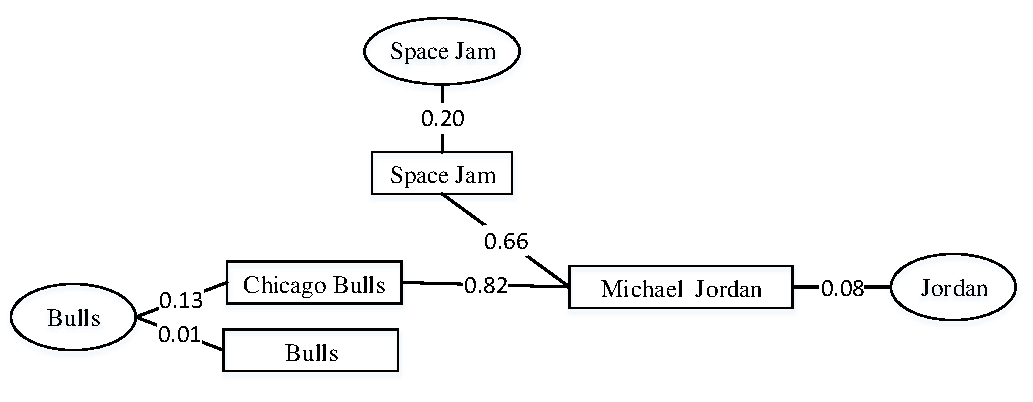
\includegraphics[height=5cm]{resource/EL_Graph_modify}
	\caption{协同推断图示例图}
	\label{fig:el_graph_modify}
\end{figure}

例如将指称项“Jordan”进行人工标注指向\textit{Michael Jordan}实体,改动后的协同推断图如图\ref{fig:el_graph_modify}所示。图中指称项“Jordan”对应的候选实体集中\textit{Michael I. Jordan}实体和\textit{Michael B. Jordan}实体对应的节点被删除,指称项“Jordan”连接到实体\textit{Michael I. Jordan}和实体\textit{Michael B. Jordan}的边被删除,另外,实体\textit{Michael I. Jordan}和实体\textit{Michael B. Jordan}节点连接到其它实体节点的边也被删除。
	
由于经过人工标注以后协同推断图发生了变化,因此对应到协同推断过程,需要根据改动以后的协同推断图对初始证据向量$s$和证据传递矩阵$T$进行改动。改动后的初始证据向量$s$和证据传递矩阵$T$如分别如公式\ref{eq:s_modify}和公式\ref{eq:T_modify}所示。
	
\begin{equation}\label{eq:s_modify}
	s=\left(0.41,0.33,0.26,0,0,0,0\right)^T
\end{equation}
	
\begin{equation}\label{eq:T_modify}
	T=
	\left(
	\begin{matrix}
	0 & 0 & 0 & 0 & 0 & 0 & 0\\
	0 & 0 & 0 & 0 & 0 & 0 & 0\\
	0 & 0 & 0 & 0 & 0 & 0 & 0\\
	1 & 0 & 0 & 0 & 1 & 0 & 0\\
	0 & 0.92 & 0 & 0.55 & 0 & 0 & 0\\
	0 & 0.08 & 0 & 0 & 0 & 0 & 0\\
	0 & 0 & 1 & 0.45 & 0 & 0 & 0\\
	\end{matrix}
	\right)
\end{equation}
	
通过观察可以发现,由于删除了部分节点,$s$和$T$的维度发生了变化,另外协同推断图边的权值变化也引起了$T$中部分值的变化。后续推断过程按照第\ref{section:collective_infer_method}节描述的方法进行即可。

\subsubsection{标注证据传播}
当人工标注指称项$m$指向目标实体$e$以后,需要将标注结果传播到同一篇文档中的其他可能共指的指称项。本文采用了两种标注证据传播方法:基于字符串完全匹配的标注证据传播方法和基于相似指称项的标注证据传播方法。

(1)基于字符串完全匹配的标注证据传播

当人工标注文档$D$中的某一个指称项$m$指向目标实体$e$以后,在文档$D$中搜索与指称项$m$名字完全相同的未标注指称项集合$M_m=\{m^{'}|Name_m=Name_{m^{'}}\}$。然后需要调整证据传递矩阵$T$中所有$m^{'}\in M_m$的指称项节点连接到其对应候选实体节点的边的权值,如公式\ref{eq:T_dupName}所示。
	
\begin{equation}\label{eq:T_dupName}
	T_{ij}=\left\{
	\begin{array}{rcl}
	1      &      & {\text{节点}j\text{对应指称项}m^{'}\text{,节点}i\text{对应实体}e}\\
	0    &      &{\text{节点}j\text{对应指称项}m^{'}\text{,节点}i\text{对应除}e\text{以外的其它实体}}\\
	\end{array} \right.
\end{equation}

(2)基于相似指称项的标注证据传播
	
当人工标注文档$D$中的某一个指称项$m$指向目标实体$e$以后,在文档$D$中搜索与指称项$m$语义相似度不小于$\alpha$的未标注指称项集合$M_m=\{m^{'}|MS(m,m^{'})>=\alpha\}$。同时依然要对证据传递矩阵$T$做调整,按照公式\ref{eq:T_simiName1}对所有$m^{'}\in M_m$的指称项节点连接到实体节点的边的权值做调整。
	
\begin{equation}\label{eq:T_simiName1}
	T_{ij}=\left\{
	\begin{array}{rcl}
	MS(m,m^{'})\times T_{ij}      &      & {\text{节点}j\text{对应指称项}m^{'}\text{,}}\\
	&	&{\text{节点}i\text{对应实体}e}\\
	(1-MS(m,m^{'}))\times T_{ij}    &      &{\text{节点}j\text{对应指称项}m^{'}\text{,}}\\
	&	&{\text{节点}i\text{对应除}e\text{以外的其它实体}}\\
	\end{array} \right.
\end{equation}
	
调整权值之后,还需要对所有指向指称项的节点$j$通过公式\ref{eq:T_simiName2}对权值做归一化处理。
	
\begin{equation}\label{eq:T_simiName2}
	T_{ij}=\frac{T_{ij}}{\sum_{k} {T_{kj}}}
\end{equation}

\section{实验结果与分析}
\subsection{实验环境}
同\ref{section:dev_env}节。

\subsection{实验数据集}
数据集同\ref{section:dataset}节,因为本章实验内容为实体链接银标准语料的辅助标注,因此不需要将数据集划分为训练集和测试集。

\subsection{实验设置}\label{section:anno_set}
本章研究主动学习方法在实体链接银标准语料构建中的作用,并验证本文提出的融合证据传播的主动学习方法对减少人工标注样本工作量的效果。实验过程中不直接使用Aida数据集的标注结果,而只使用模型选择的待标注样本的标注结果。本章设计了以下六个对比实验:

(1) 以顺序标注方法作为基线方法,评价标注过程中,语料中指称项链接的正确率的变化,同下列基于主动学习的标注方法做比较。

(2)以最大不确定度的指称项选择法选择待标注指称项,在标注证据传播过程中,不对当前标注结果进行传播。

(3))以最大不确定度的指称项选择法选择待标注指称项,在标注证据传播过程中,基于字符串完全匹配对当前标注结果进行传播。

(4) 以最大不确定度的指称项选择法选择待标注指称项,在标注证据传播过程中,基于相似指称项对当前标注结果进行传播。

(5)以基于同名指称项的最大标注回报选择法选择待标注指称项,在标注证据传播过程中,基于字符串完全匹配对当前标注结果进行传播。

(6)以基于相似指称项的最大标注回报选择法选择待标注指称项,在标注证据传播过程中,基于相似指称项对当前标注结果进行传播。

\subsection{实验结果与分析}
\begin{figure}[!htb]
	\centering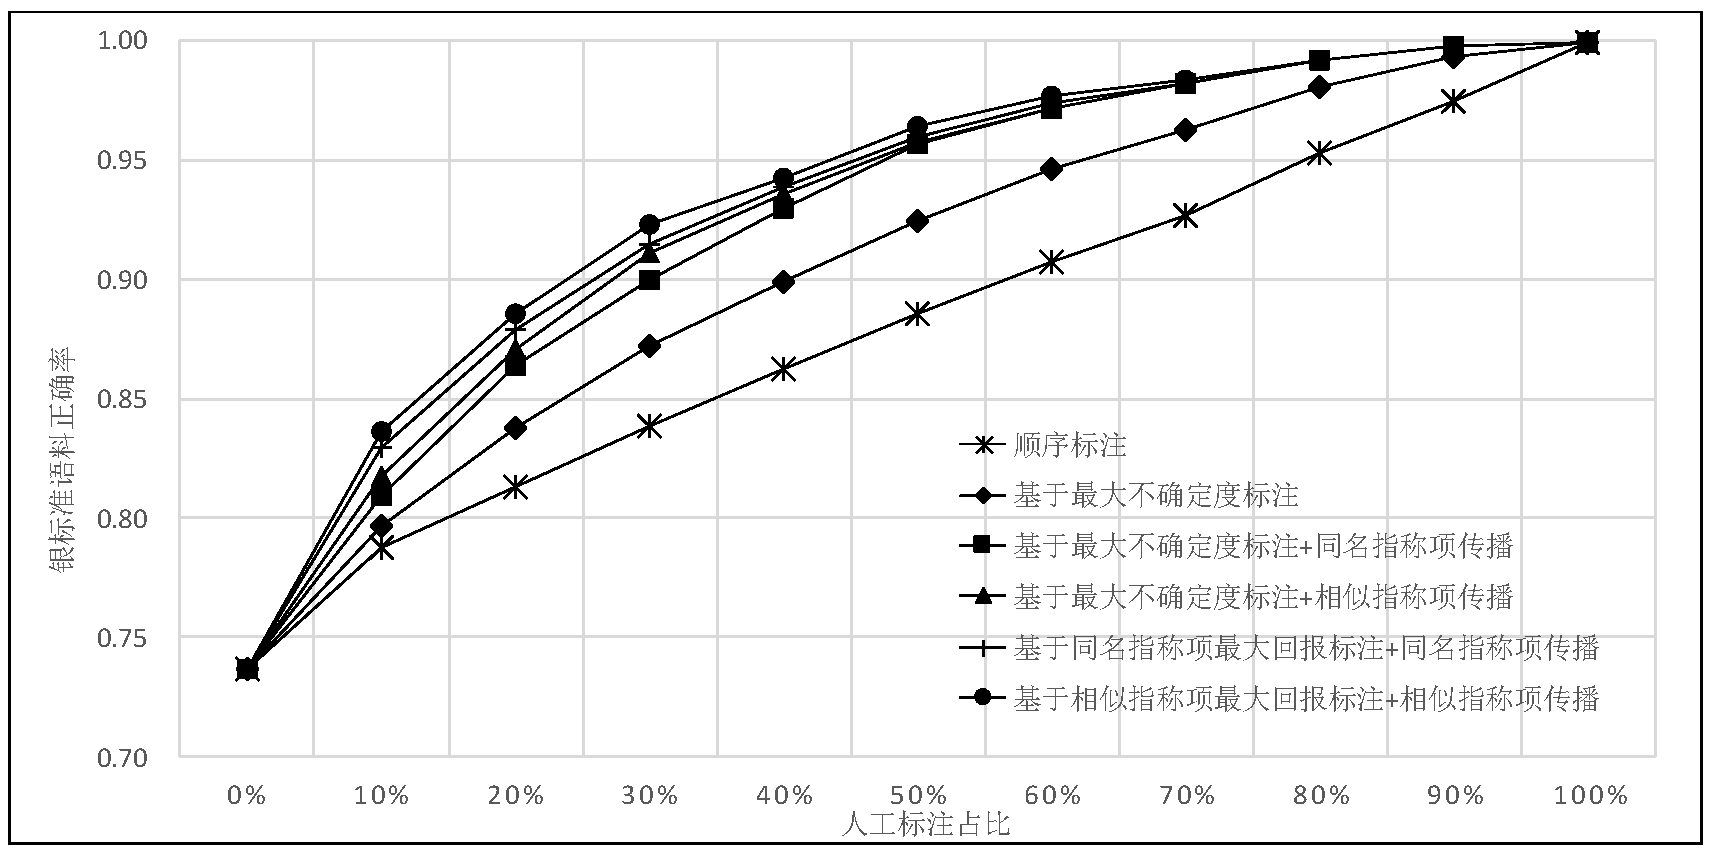
\includegraphics[height=8cm]{resource/anno_result}
	\caption{银标准语料库构建实验结果}
	\label{fig:anno_result}
\end{figure}

本文实验环节测试了上述六种标注方式在数据集上的标注效果。如图\ref{fig:anno_result}所示。顺序标注并且没有对标注证据进行传播的方法,标注效率是最低的。以最大不确定度的指称项选择法选择待标注指称项,在不进行标注证据传播的情况下,标注效率明显优于顺序标注的方式。这是因为该基于主动学习的方法能够有效搜索出预标注不确定度大的样本,保证交由人工标注的样本很可能是预标注错误的样本,从而提高标注效率,并且这一假设通过实验得到了证明。

以最大不确定度的指称项选择法选择待标注指称项,并基于同名指称项和基于相似指称项的方式对当前标注结果进行标注证据传播,观察曲线可以发现,相比于不对标注证据传播的方式,标注效率得到了显著提升,并且基于相似指称项的方式优于基于字符串完全匹配的方式。这是因为,同一文档中相同指称存在多次出现的情况,基于同名指称项的标注证据传播能利用一次标注提高多个未标注指称项的链接正确率。另外,基于相似指称项的证据传播方式能将标注结果传播到存在共指关系的未标注指称项,因此比基于同名指称项的标注证据传播方法性能更好。实验证明,在实体链接银标准语料标注任务中,融合标注证据传播,对提升主动学习方法的性能有显著的效果。

在待标注样本选择阶段,基于同名指称的最大标注回报选择法和基于相似指称的最大标注回报选择法,相比最大不确定度的指称项选择法,标注效率得到提升。提升的原因是,在样本选择的阶段,不仅考虑到单个指称项的预测链接不确定度,还考虑了标注该指称项对文档中其它存在共指关系的指称的影响。

综合分析实验结果数据,在仅标注50\%的指称项时,顺序标注的方式只能将语料库标注正确率提升到88.6\%,而以基于相似指称的最大标注回报选择法选择待标注指称项,在标注证据传播过程中,基于相似指称项对当前标注结果进行传播的方法,标注正确率提升到了96.4\%。

\section{本章小结}
本章介绍了一种基于主动学习的实体链接银标准语料库构建方法。并且,本文基于实体链接任务的特点,对已有的主动学习方法进行了改进,包括引入了基于标注回报率待标注样本选择的评价方式,以及加入了标注样本的证据传播方法,提升了主动学习方法的性能。在本章实验环节,本文对提出的这些方法进行了验证,并分析了实验结果。